\chapter{Implementation}
\label{chp:implementation}
This chapter explains how the hybrid vehicle, which is similar to the Toyota Prius second generation, was modelled in Simulink. Then the implementation details in Matlab of each of the six game-theoretical approaches are described.

\section{Hybrid Vehicle Model}
The model of the hybrid vehicle is split into different controllers and each of them is responsible for controlling the corresponding part of the hybrid. The chapter describes the Drive Cycle Controller, the Power Controller, the Gasoline Engine Controller, the Electric Motor Controller, the Gearbox and the Vehicle dynamics. The game-theoretical logic is included in the Power Controller, which is the principal controller where the solution is computed. It is shown in the next section.

\subsection{Drive Cycles Controller}
This subsection deals with the demand of speed which comes from the Drive Cycle and how it is transformed to acceleration demand, which corresponds to the acceleration pedal in a vehicle.

Two different drive cycles were simulated. The FTP-75 drive cycle is intended to test light-duty vehicles in the U.S. and measure their gas emissions and fuel economy. It lasts for 1874s, the total distance it covers is 17.77km and the average speed is 34.1 km/h. The drive cycle contains three phrases - cold start from 0-504s, transient phase from 505-1369s and hot start from 1370-1874. The last phase is exactly the same as the first phase. Figure \ref{fig:ftp75} shows the time and speed of this drive 
cycle.

\begin{figure}[h]
\centering
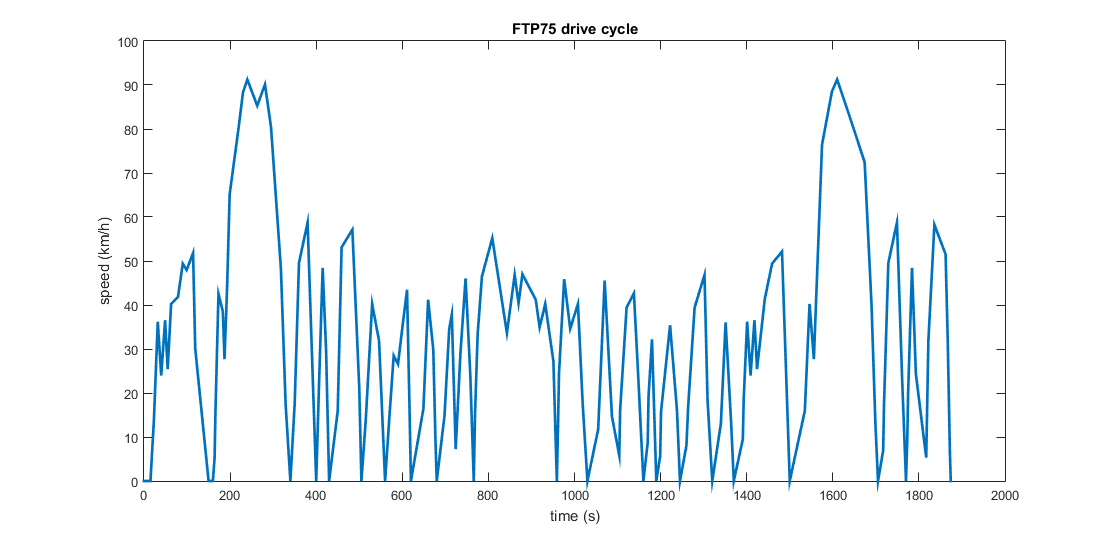
\includegraphics[scale=0.45]{figures/FTP75}
\caption{FTP drive cycle}
\label{fig:ftp75}
\end{figure}

The NEDC drive cycle was invented to test light-duty cars in Europe. Its duration is 1180s, the distance is 11.02km and the average speed 33.6km/h. It contains four equivalent urban driving phases called ECE-15. They last from 0-780s and there is also a fourth highway driving phase called EUDC from 781-1180s. Figure \ref{fig:nedc} shows the time versus the speed in the NEDC drive cycle.

\begin{figure}[h]
\centering
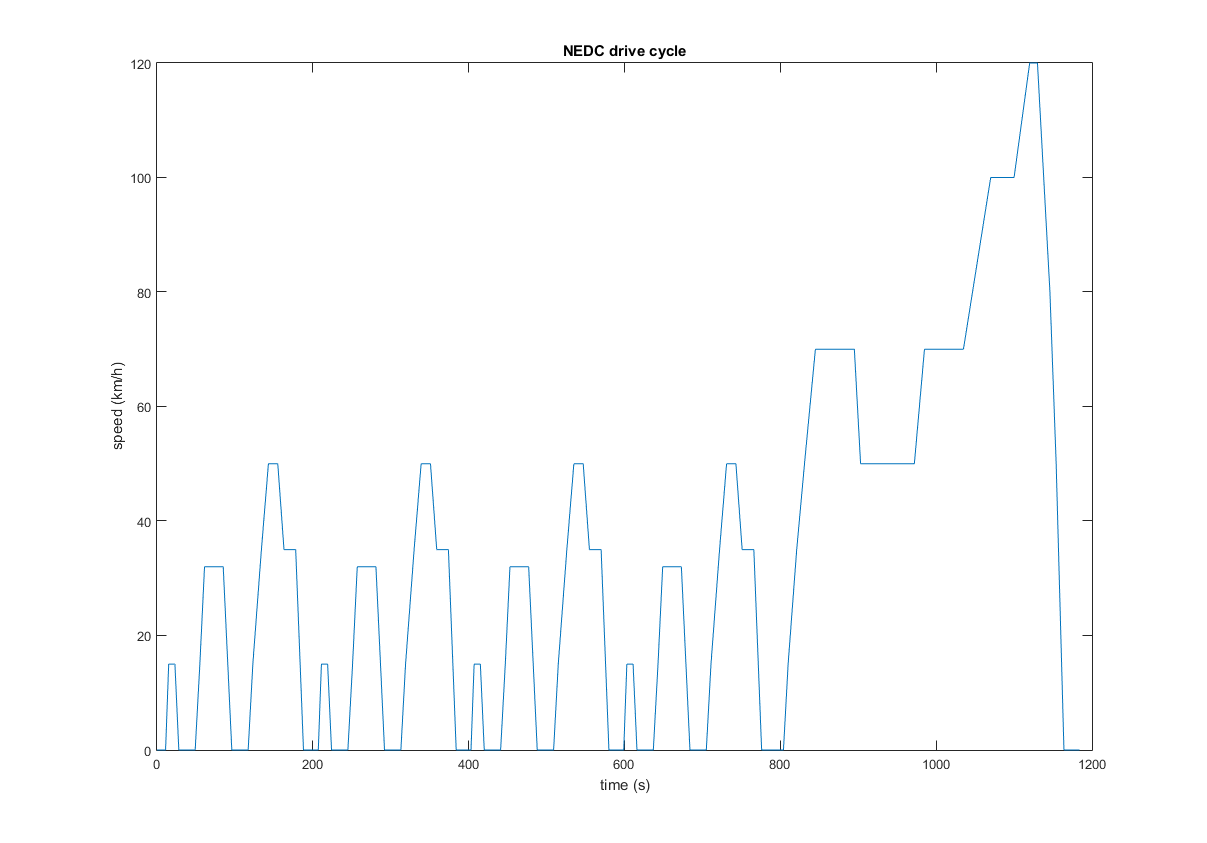
\includegraphics[scale=0.45]{figures/NEDC}
\caption{NEDC drive cycle}
\label{fig:nedc}
\end{figure}

The Speed Control block takes as input the demanded speed from the drive cycle and the actual speed of the vehicle both in \textit{km/h} and calculates as output the acceleration which lies between -1 and 1 where a negative value means braking and a positive value means acceleration. A value of 0 corresponds to cruising or maintaining a constant speed. In order to calculate the acceleration demand, the difference between the demanded and actual speed is taken.

\subsection{Power Controller}
The Power Controller takes as input the acceleration demand $a$ and the state of charge $SOC$ of the battery which comes from the Electric Motor Controller. In order to transform the acceleration demand into torque demand $\tau_{dem}$, the acceleration is scaled by the maximum torque of 400 \textit{Nm} which can be requested. This value was chosen since this is the maximum output torque of the Toyota Prius electric motor. The minimum demanded torque is -400 \textit{Nm} which corresponds to deceleration. The current motor speed $\omega_{mot}$ is mapped to the torque of the motor which it is capable of generating at this moment. This value is taken as upper limit and its negated value is taken as a lower limit of the torque. 

There are two subsystems in the Power Controller, the Battery Management and the Game Theory Controller. The first of them takes as input the battery $SOC$, its current in \textit{A}, its voltage in \textit{V} and computes the required recharge power $P_{batReq}$ and the battery limit $P_{batLim}$. The recharge power is requested when the SOC of the battery lies between 40 and 60\%. If the SOC falls below 40\% then the battery is forced to be recharged even if that means not meeting the drive cycle requirements and not achieving the demanded speed. After the battery has been charged up to 60\%, the recharging stops and the requested battery power is set to 0. The battery limit calculation takes into account that the maximum voltage of the battery is 200V and that its maximum power is 21 kW.

The Game Theory Controller is the primary place where the computation of the solution to the power distribution problem happens. The outputted demanded torque $\tau_{dem}$ is fed into the Game Theory Controller block. In addition, the other inputs of this block are required power, which is:
\begin{equation}
P = \tau \times \omega
\end{equation}
where power $P$ is in \textit{W}, torque $\tau$ is in \textit{Nm} and the velocity $\omega$ is angular \textit{rad/s}.
The Game Theory Controller also receives the battery SOC in \%, the generator $\omega_{gen}$, engine $\omega_{eng}$, motor $\omega_{mot}$ speeds all in \textit{rad/s}, the Total Fuel consumed up to this moment from the beginning of the drive cycle $TF$ in \textit{litres}, the battery limit and the required battery recharge power $P_{batReq}$ as described in the Battery Management subsystem above. The Game Theory Controller block contains the game-theoretical logic embedded as a Matlab function. Apart from it, it also regulates the speed of the engine by taking the difference between the required driving power $P_{drive}$ and the recharge power for the battery $P_{batReq}$. The resulting power is given as an input to a lookup table to find the corresponding engine speed in \textit{rpm}. To obtain the Generator torque $\tau_{gen}$ the engine torque and the generator speed $\omega_{gen}$ in \textit{rad/s} are taken. If the motor needs to provide additional power for the battery, this power is taken to be the sum of the battery available power and the generator power. The battery available power $P_{batAv}$ is computed in a separate subsystem using the engine torque $\tau_{eng}$, speed $\omega_{eng}$ and power $P_{eng}$, battery recharge power $P_{batReq}$ and battery limit $P_{batLim}$. 
Four values come as a result from the Game Theory Controller, the engine throttle $\theta$, the motor torque $\tau_{mot}$, the generator torque $\tau_{gen}$, the reference engine speed in \textit{rpm} $\omega_{eng}$. These are fed to a final Speed Controller block for controlling the engine speed which outputs the final engine throttle $\theta$ as percentage from the maximum possible torque of the engine $\tau_{engMax}$.

\subsection{Engine Controller}
The Engine Controller receives the throttle in \% as input and sends the torque as output. 

The Gasoline Engine library block implements a gasoline fuel engine and its speed controller. Firstly, the masked library block and then the extensions added to it to will be explained. The input signal between 0 and 1 indirectly controls the engine speed. Whenever the input is outside of the allowed range it is limited to 0 or 1 respectively. The mapping of speed in \textit{rpm} to torque in \textit{Nm} is implemented as a 1D lookup table. The throttle goes through a Switch block which ensures that the maximum speed of the engine is not exceeded. If this happens, the throttle is set to 0. Otherwise the torque and the angular velocity are measured. The torque flows to the output. The angular velocity measured in \textit{rad/s} is fed to the lookup table in \textit{rpm} to find the corresponding torque and it is also given to the switch block for controlling the maximum speed.

An additional functionality which was implemented to extend the library block was to limit the torque from 0 to 136 and also speed from 0 to 6000 rpm. Figure \ref{fig:engineTorqueSpeed} shows the torque speed curve of the engine. It provides maximum torque of 136 in the speed range 2800 - 3100 rpm. For this reason when the acceleration is constant and the engine provides maximum torque, there is a discrepancy in the simulation results, because the speed keeps jumping from 2800 to 3100 quickly, which is inefficient. Therefore, a hysteresis was implemented by a Relay block which has a switch on and a switch off point values. When the signal lies between 2800 and 3100 rpm it is either set to 2800 or to 3100 rpm to prevent such jittering.

A Driveline environment is connected to the output of the Gasoline Engine block which provides the simulation environment. Torque and angular velocity are measured and given to a Scope block for displaying the results of the engine. Power is also calculated by taking the product of torque and velocity.

A separate subsystem is responsible for the fuel and gas emissions calculations. It receives the engine speed in \textit{rpm} and the torque and outputs Total Fuel $TF$ in \textit{l}, Fuel Consumption $FC$ in \textit{l/100km}, CO emissions, HC emissions, NOX emissions all in \textit{g/km}. For their calculation 1D lookup tables are used, which hold the data for the gas emissions in grams per second \textit{g/s}. To transform \textit{g/s} into \textit{g/km} the total distance travelled is required. For this the average speed of the drive cycle is calculated and is multiplied with the total time. 

\subsection{Electric Motor Controller}
The Electric Motor Controller receives as input the demanded motor torque and generator torque. It outputs the battery characteristics and the actual motor torque and generator torque.

The battery is modelled by a Battery block of a Nickel-Metal-Hydride type. The nominal voltage is 200V and the rated capacity is 6.5Ah. At the beginning of the simulation the battery is fully charged, its state of charge is set to 100\%. The discharge characteristics are shown in Figure \ref{fig:batteryDischarge}. The first figure shows the nominal discharge current and the second shows the discharge curves at the specific discharge currents. The discharge model $f_1$ and charge model $f_2$ of the battery are \citep{batteryMatlab}:

\begin{equation}
\begin{split}
f_1(it,i*,i,Exp) = E_0 - K \cdot \frac{Q}{Q-it} \cdot i* - K \cdot \frac{Q}{Q-it} \cdot it + Laplace^{-1} \bigg( \frac{Exp(s)}{Sel(s)} \cdot 0 \bigg)
\end{split}
\end{equation}

\begin{equation}
\begin{split}
f_2(it,i*,i,Exp) = E_0 - K \cdot \frac{Q}{|it|+0.1 \cdot Q} \cdot i* - K \cdot \frac{Q}{Q-it} \cdot it + Laplace^{-1} \bigg( \frac{Exp(s)}{Sel(s)} \cdot \frac{1}{s} \bigg)
\end{split}
\end{equation}
where $E_0$ is the constant voltage, $Exp(s)$ is the exponential zone dynamics in $V$, $Sel(s)$ is the battery mode, 0 for discharging and 1 for charging, $K$ is polarization constant in $Ah^{-1}$, $i*$ is the low frequency current dynamics in $A$, $i$ is the battery current in $A$, $it$ is the extracted battery capacity in $Ah$, $Q$ is the maximum battery capacity in $Ah$.

\section{Game-theoretical algorithms}
This chapter describes the implementation of all six game-theoretical approaches in Matlab.